\section{Lecture 29 - 11/14/2022}

\subsection{Harmonicity}

In this lecture, we will continue finishing the proof that $\text{wMVP}_2 \implies $ Harmonic. First, we will prove the following theorem that will be vital in showing this implication:

\begin{theorem}[Global Maximum Principle]
Suppose $u \in \text{wMVP}_2(\Omega) \cap C(\Omega)$, where $\Omega$ is a domain. If $u$ has a local minimum at $z_0 \in \Omega$, then $u(z) \equiv u(z_0)$ is identifically constant.
\end{theorem}

\begin{proof}
    We will prove this using a continuous induction! Indeed, let
    \[A \coloneqq \{z \in \Omega\ |\ u(z) = u(z_0)\} = u^{-1}(\{u(z_0)\})\]
    Clearly $z_0 \in A$ and $A$ is closed. Now to show that $A$ is open, let $z \in A$.\\\\
    Since $z \in A$, we know that $u(z) = u(z_0) \geq u(\xi)$ for all $\xi \in \Omega$, hence $u$ has a global (so local) maximum at $z$.\\\\
    Then, by the Local Maximum Principle, there exists some $r > 0$ such that $u(\xi) = u(z)$ for all $\xi \in D_{z, r} \subset A$. So $A$ is open.\\\\
    Since $\Omega$ is connected, we conclude that $A = \Omega$
\end{proof}

\begin{theorem}
    Let $\Omega$ be a domain, suppose $u \in \text{wMVP}_2(\Omega) \cap C(\Omega)$, then $u \in \text{Harm}(\Omega)$. 
\end{theorem}

\begin{proof}
    It suffices for us to verify this on disks $D_{z_0, R}$ such that $cl(D_{z_0, R}) \subset \Omega$. Indeed, let $\varphi$ be the function
    \[\varphi \coloneqq u - v\]
    , where $v \in \text{Harm}(D_{z_0, R}) \cap C(\overline{D_{z_0, R}}^{cl})$ such that
    \[v|_{\partial D_{z_0, R}} = u|_{\partial D_{z_0, R}}\]
    We can construct $v$ by taking boundary values of $u$ and take its Poisson extension on $D_{z_0, R}$. We claim that it is actually the case that $\varphi \equiv 0$.\\\\
    First we note that
    \[\pm \varphi \in \text{wMVP}_2(D_{z_0, R}) \cap C(\overline{D_{z_0, R}}^{cl})\]
    \[\pm \varphi \in \text{wMVI}_2(D_{z_0, R})\]
    Let $M$ be the maximum (this exists as the closure of the disk is compact),
    \[M \coloneqq \max_{z \in \overline{D_{z_0, R}}^{cl}} \varphi(z)\]
    Suppose $M > 0$, then $M$ is not attained at the boundary because $\varphi$ is identically $0$ on the boundary, but this means that $M$ is attained at $z_1 \in D_{z_0, R}$. By the Gloval Maximum Principle, $\varphi(z) \equiv M$ on $D_{z_0, R}$. Then by continuity this means that $\varphi$ attains $M$ on the boundary, which is a contradiction!\\\\
    If we replace $\varphi$ by $-\varphi$, we also find that $M$ cannot be negative.\\\\
    But this means that $M = 0$, so the Global Maximum Principle tells us that $\varphi$ is identically $0$, so we are done.
\end{proof}

\subsection{Reflection Principles}

There're some particularly useful corollaries of the theorem, known as the reflection principle!

\begin{corollary}[Reflection Principle for Harmonic Functions]
    Let $\Omega = \Omega^*$, where $\Omega^*$ denote the complex conjugation of $\Omega$. In other words, $\Omega$ is a \textbf{symmetric domain}.\\\\
    Define $\Omega^+ \coloneqq \Omega \cap \Cbb_+ = \{z \in \Omega: Im(z) > 0\}$ and $\Omega^- \coloneqq \Omega \cap \Cbb_-$ similarly, let $u \in \text{Harm}(\Omega^+)$ such that for all $\xi \in \Rbb \cap \Omega)$, $\lim_{z \to \xi} u(z) = 0$, then the following function
    \[\Tilde{u}(z) \coloneqq \begin{cases}
    u(z),\ z \in \Omega^+\\
    -u(\overline{z}),\ z \in \Omega^-\\
    0,\ z \in \Rbb \cap \Omega
    \end{cases}\]
    Then, $\Tilde{u} \in \text{Harm}(\Omega)$
\end{corollary}

\begin{proof}
It suffices for us to show that $\Tilde{u}$ is continuous and $\text{wMVP}$ (doesn't matter if it's $1$ or $2$) over $\Omega$, then our prior theorems imply that $\Tilde{u}$ is harmonic over $\Omega$.\\\\
Clearly, $\Tilde{u} \in C(\Omega)$ by the Glueing Lemma.\\\\
Now for $\text{wMVP}$, if $z_0 \in \Omega^+ \cup \Omega^-$, then $\text{wMVP}$ holds by harmonicity of $u$ and $-u$. Now, if $z_0 \in \Rbb \cap \Omega$, then we note that
\[\frac{1}{\pi r^2} \int_{D_{z_0, r}} \Tilde{u(z)} dA(z) = 0\]
by symmetry, so $\Tilde{u}$ is $\textbf{wMVP}$ on $z_0$.
\end{proof}

Our reflection principle can also be shown for analytic functions!

\begin{theorem}[Reflection Principle for Analytic Functions]
    Define $\Omega = \Omega^*$, $\Omega^+$, and $\Omega^-$ as before, and suppose $f \in \text{Hol}(\Omega^+)$ such that for all $\xi \in \Rbb \cap \Omega$,
    \[f(\xi) \coloneqq \lim_{z \to \xi} f(z) \in \Rbb\]
    Then the following function
    \[\Tilde{f}(z) \coloneqq \begin{cases}
    f(z),\ z \in \Omega^+\\
    \overline{f(\overline{z})},\ z \in \Omega^-\\
    f(z),\ z \in \Rbb \cap \Omega
    \end{cases}\]
    , then $\Tilde{f} \in \text{Hol}(\Omega)$
\end{theorem}

\begin{proof}
    We can show this using Morera's Theorem. In fact, recall in a previous homework exercise, we had that:
\[\noindent\fbox{%
    \parbox{\textwidth}{%
\begin{exercise}
        Let $L$ be a line in the complex plane. Suppose $f(z)$ is a continuous complex-valued function on a domain $D$ that is analytic on $D \setminus L$. Show that $f(z)$ is analytic on $D$.
    \end{exercise}
    }%
}\]
\end{proof}

\begin{remark}
    The conclusion of the reflection principle for analytic functions is still true if we only assume that
    \[\lim_{z \to \xi} Im(f(z)) = 0\]
    We can also replace the line in both reflection principles with a circle! For harmonic functions, this is because harmonic maps are invariant under conformal maps.
\end{remark}

While reflection about lines and circles are all global extensions, we also have a notion of local extensions in what's known as \textbf{analytic curves}

\begin{definition}
    $\gamma$ is an \textbf{analytic curve} if locally it is a continuous image of a diameter of a disc, ie:
     \[\fbox{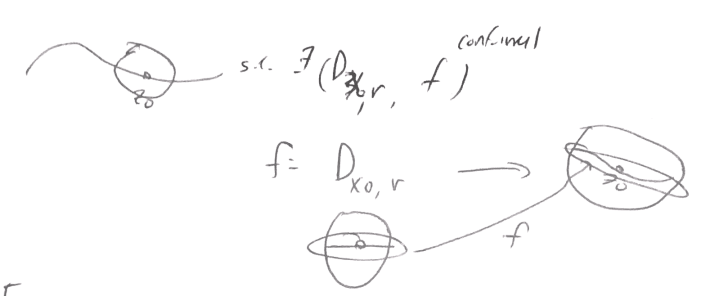
\includegraphics[width=.8\textwidth]{Figures/curve.png}}\]
     For all $z_0 \in \Gamma$, there exist some neighborhood $N$ around $z_0$ and $(D_{x_0, r}, f)$ such that $f$ maps the diameter of $D_{x_0, r}$ to $N \cap \gamma$.
\end{definition}

\begin{example}
    The ellipse $\frac{x^2}{a^2} + \frac{y^2}{b^2} = 1$ is an analytic curve.
\end{example}

The main idea behind reflection across analytic curves is as follows:\\\\
Suppose $\Omega$ is some domain where $\partial \Omega$ is an analytic curve:
\[\fbox{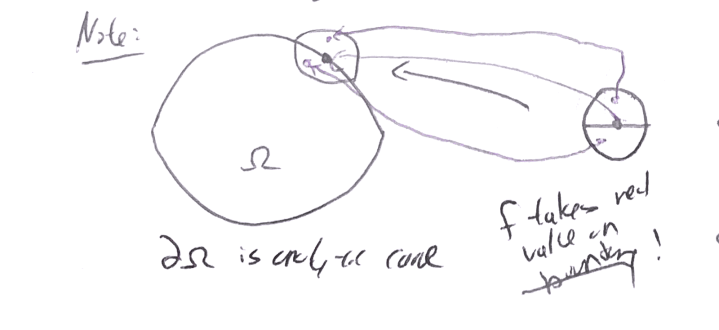
\includegraphics[width=.8\textwidth]{Figures/extension.png}}\]
The symmetry in the disk induces a symmetry near $\partial \Omega$, so we can extend it locally and use the reflection principle.

\begin{proposition}
Harmonic functions are real-analytic, meaning that the function is locally representable in power series as
\[(x - x_0)^n \cdot (y - y_0)^m\]
Or equivalently as power-series:
\[(z - z_0)^k (\overline{z - z_0})^\ell\]
\end{proposition}

\begin{proof}
    Recall the Poisson Formula lets you write a harmonic function $u(z)$ as
    \[u(z) = \int_{\mathbb{T}} f(\xi) \frac{d\xi}{2\pi} + \sum_{k > 0} z^k \int f(\xi) \overline{\xi}^k \frac{|d\xi|}{2\pi} + \sum_{k > 0} \overline{z}^k \int f(\xi) \xi^k \frac{|d\xi|}{2\pi}\]
    Applying a change of coordinates, we can reconstruct the power series based on harmonic values od disks.
\end{proof}